% Source PDF pages 235--242, printed pages 213--220.
\OriginalPage{213}{Implementing smpl}
\setcounter{chapter}{8}
\setcounter{section}{0}
\noindent{\LARGE\bfseries 8.\quad Implementing \textbf{smpl}\par}
\label{chap:implementing-smpl}
\section{Introduction}

In this chapter, we'll take a close look at the design and implementation
of \textbf{smpl}. A detailed understanding of how \textbf{smpl} works will plug any gaps left
by Chapter 2, help you fix it if it breaks, and provide a basis for tailoring
and extending it to meet needs unique to your environment. We'll look at
some possible extensions in the next chapter.

This implementation of \textbf{smpl} uses the C language as described by
Kernighan and Ritchie in \textit{The C Programming Language} [K\&R].\footnote{This departure from our usual reference notation is in deference to the industry-wide recognition of ``K\&R''.}
If C is a new programming language for you, you may find a more extensive
introduction, such as that provided by Gehani [1985], to be a helpful
supplement to [K\&R]. For reference purposes, the book by Harbison and
Steele [1984] is excellent. The implementation presented here is straightforward:
the code should be easy to read even for the reader new to C.
Traditional arrays and indexes are used for data structures, rather than C
structures and pointers, to maintain correspondence between this version of
\textbf{smpl} and versions implemented in other languages.

The Appendix provides C source code listings for the following files:
\begin{description}
\item[\textit{smpl.c} ---] the \textbf{smpl} simulation subsystem except for random variate generation functions,
\item[\textit{rand.c} ---] random variate generation functions,
\item[\textit{smpl.h} ---] \textbf{smpl} external name declarations and various user-level directives, and
\item[\textit{stat.c} ---] normal and $t$ distribution quantile functions.
\end{description}


\OriginalPage{214}{Implementing smpl}
\begin{figure}[H]
\centering\small
\begin{tabular}{@{}ll@{}}
\multicolumn{2}{@{}l}{\textbf{initialization}}\\
\texttt{smpl()*} & initialize simulation subsystem\\
\texttt{reset()*} & clear measurement counters and accumulators\\[3pt]
\multicolumn{2}{@{}l}{\textbf{namespace and element pool allocation}}\\
\texttt{save\_name()} & save model or facility name\\
\texttt{mname()*} & return model name pointer\\
\texttt{fname()*} & return facility name pointer\\
\texttt{get\_blk()} & allocate block of elements\\
\texttt{get\_elm()} & allocate single element\\
\texttt{put\_elm()} & deallocate single element\\[3pt]
\multicolumn{2}{@{}l}{\textbf{event scheduling}}\\
\texttt{schedule()*} & schedule event\\
\texttt{cause()*} & cause event and advance simulation time\\
\texttt{time()*} & return current simulation time\\
\texttt{cancel()*} & cancel scheduled event\\
\texttt{suspend()} & remove event list entry of preempted token\\[3pt]
\multicolumn{2}{@{}l}{\textbf{list processing}}\\
\texttt{enlist()} & enter element in queue or event list\\[3pt]
\multicolumn{2}{@{}l}{\textbf{facility definition, operation, and query}}\\
\texttt{facility()*} & define facility\\
\texttt{resetf()} & clear facility and queue measurements\\
\texttt{request()*} & reserve facility (non-preemptive)\\
\texttt{enqueue()} & build facility queue entry\\
\texttt{preempt()*} & reserve facility (preemptive)\\
\texttt{release()*} & release facility and reinitiate queued request\\
\texttt{status()*, inq()*} & return current facility status, current queue length\\
\texttt{U()*, B()*, Lq()*} & return utilization, mean busy period, mean queue length\\[3pt]
\multicolumn{2}{@{}l}{\textbf{debugging and reporting}}\\
\texttt{trace()*} & turn trace on/off\\
\texttt{msg()} & display/print trace message\\
\texttt{end\_line()} & trace line end: test for and process page end\\
\texttt{pause()*} & pause execution\\
\texttt{error()*} & print/display error message and halt\\
\texttt{report()*} & generate simulation report\\
\texttt{reportf()*} & generate facilities report\\
\texttt{rept\_page()} & generate facility report page\\
\texttt{lns()*} & count output lines used on current page\\
\texttt{endpage()*} & advance (pause) on full page (screen)\\
\texttt{newpage()*} & initialize line count for new page or screen\\
\texttt{sendto()*} & set/get current output destination
\end{tabular}
\caption{\textit{smpl.c} Functions}
\end{figure}


\OriginalPage{215}{8.2 The Element Pool and Namespace}
The random variate functions are logically part of \textbf{smpl}, but are maintained
in a separate file and separately compiled as a matter of convenience. The
\textit{smpl.h} file is provided for inclusion in simulation programs; in addition to
external name declarations, it contains \texttt{\#include}'s for \textit{stdio.h} and \textit{math.h},
and \texttt{typedef} and \texttt{\#define} for \texttt{real} and \texttt{then}. The \textit{stat.c} file is used by the
batch means analysis module of Section 4.7, and won't be discussed here. If
you have \textbf{smpl} in machine-readable form, you may want to print the source
files to avoid flipping back and forth between this chapter and the
Appendix as we look at what the various \textbf{smpl} functions do.

\textit{smpl.c} contains 37 functions, 26 of which can be called from a simulation
program. Function names are listed in Figure 8.1, categorized by use. Names
of user-callable functions (names not declared \texttt{static}) are marked with an
asterisk: most of these were discussed in Chapter 2 and should be familiar.
Function names in Figure 8.1 appear in the same order as functions in the
\textit{smpl.c} listing in the Appendix. Our discussion will stray from this order
somewhat to follow order of use: we'll begin with a look at the basic
building block used to form \textbf{smpl} data structures.

\section{The Element Pool and Namespace}

One of the design goals for \textbf{smpl} was compactness. This was motivated in
part by the limited memory sizes --- as small as 32K bytes --- available for
some implementations, and in part by the use of \textbf{smpl} as a ``kernel'' of a larger
application-oriented simulation system. Examples of the latter include
highly-parameterized configurable local area network and computer system
simulation models.

Compactness is achieved in part through the use of a single basic data
element for all \textbf{smpl} data structures. This element comprises five fields,
typed and named as shown below.\footnote{In the source code, these fields are named using a lower-case ``l''. In the text and figures, an upper-case ``L'' is used to avoid confusion between ``l'' and ``1''.}

\begin{center}
\begin{tabular}{|c|c|c|c|c|}\hline
L5 & L4 & L3 & L2 & L1 \\ \hline
\multicolumn{2}{c}{real} & \multicolumn{3}{c}{integer}
\end{tabular}
\end{center}

\textbf{smpl} maintains a pool of these elements; elements are allocated from this
pool to construct facility descriptors, queue entries, and event list entries.

\OriginalPage{216}{Implementing smpl}
\noindent They also are used to construct table and storage descriptors, as we'll see in
the next chapter.

\textit{smpl.c} declares the integer fields L3--L1 to be of type \texttt{int}. On some
machines, \texttt{int}s are 16-bit quantities (15 bits plus sign) and the maximum
value which can be represented by this type is only 32767: on other machines
(or in other C implementations), \texttt{int}s are 32-bit quantities. Certain fields
are used for counts (e.g., in a facility descriptor, L3 is a count of the number of
releases): the maximum count is limited to the maximum \texttt{int} value, which
may limit the length of a simulation run. While \texttt{reset()} can be used to reinitialize
counts when this limit is reached, you may want to consider
defining integer fields as type \texttt{long} in this case. This concern, of course,
applies to the simulation program as well as to \textit{smpl.c}. In the author's
environment, simulation models can be run on both microcomputers with 16-
bit \texttt{int}s and mainframe computers with 32-bit \texttt{int}s; long runs can be done on
the mainframe system, so everything works out nicely.

Elements are declared as a set of arrays of fields (see the global
declarations in \textit{smpl.c}); element \texttt{Ln[0]} is unused. The element pool takes
two forms, as shown in Figure 8.2: each has its own mode of allocation.
During model initialization, the pool is viewed as an array of elements from
which contiguous blocks are allocated to construct facility (or table or
storage) descriptors; \texttt{blk} is the index of the next available element. When
model initialization is complete, the remaining elements in the pool are
linked together in a list: \texttt{avl} is the index of the element at the head of this
list. During simulation, elements from this list are dynamically allocated
and deallocated as events are scheduled and caused and tokens are queued
and dequeued.

The size of the element pool is determined by the value defined for \texttt{nl}.
A facility descriptor for an $n$-server facility requires $n+2$ elements, each
queue entry requires 1 element, and each scheduled event requires 1 element.
Generally, a token either will have an event scheduled for it or will be
queued, so the maximum number of elements needed for queue and event list
entries is equal to the maximum number of tokens. Thus, a value for \texttt{nl} of 128
is sufficient for models with 16 single-server facilities and up to 79 tokens.

One other global array is declared in \textit{smpl.c}: the character array
\texttt{name[]}. This array, called namespace, is used to record model and facility
(and table or storage) name strings. \texttt{avn} is the index of the next available
namespace position, and \texttt{ns} determines namespace size. \textbf{smpl} limits model
names to 50 characters, single-server facility names to 17 characters, and
multi-server facility names to 14 characters. (The shorter limit for a multi-
server facility name is to insure space to append the number of servers in the
facility report.)


\OriginalPage{217}{8.3 Initialization}
\begin{figure}[H]
\centering
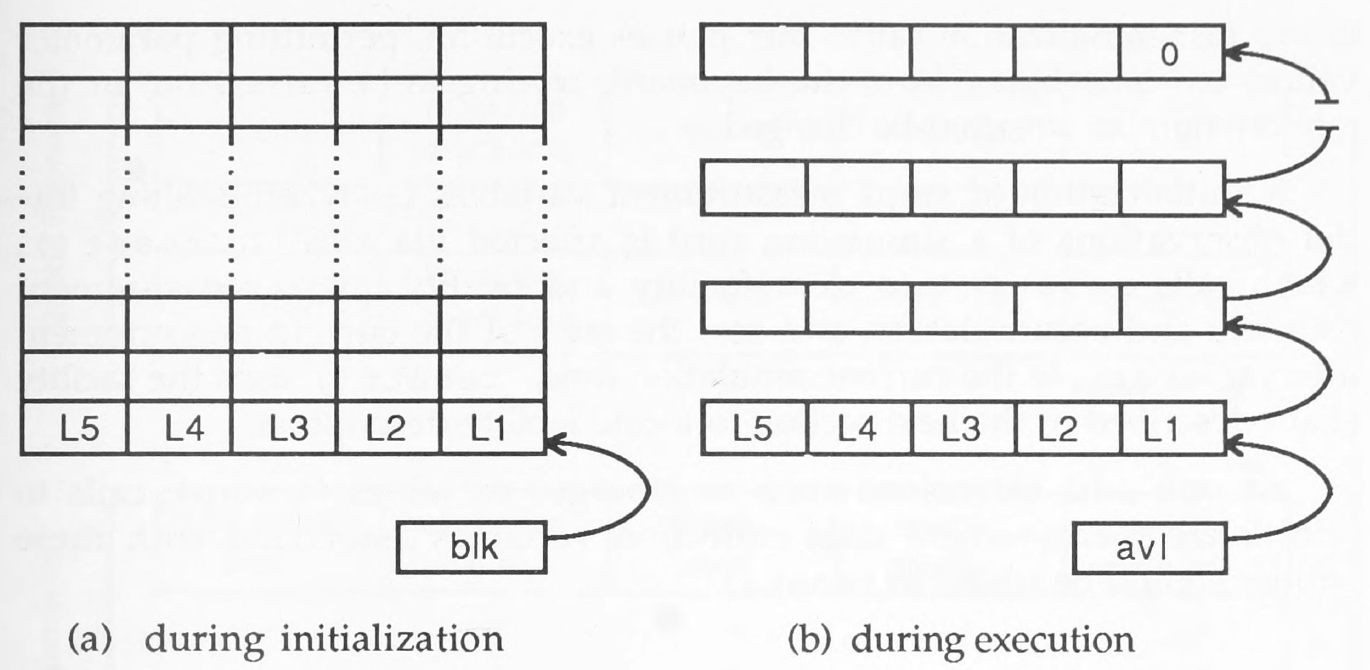
\includegraphics[width=.72\textwidth]{figures/ch8-figure-8-2.png}
\caption{The \textbf{smpl} Element Pool}
\end{figure}

\section{Initialization}

The simulation subsystem is initialized via a call to \texttt{smpl()} with parameters
\texttt{m} and \texttt{s}: \texttt{m} controls \textbf{mtr} activation and \texttt{s} is a pointer to a character
string containing the model name. \textbf{mtr} is part of the SMPL simulation
environment; some of its facilities were described in the previous chapter.
While its implementation isn't included here, an overview of its design is
given in Chapter 9, and you may want to build similar facilities into your
system. The ``hooks'' between \textbf{smpl} and \textbf{mtr} have been left in place (in the
form of comments) in the source code in the Appendix, and their functions
will be noted as we encounter them.

\texttt{smpl()} initializes various indexes, sets the simulation time (\texttt{clock})
and the start of the current measurement interval (\texttt{start}) to zero, clears the
element pool, and saves the model name in namespace. Names are stored in
namespace by \texttt{save\_name()}, which limits a name to a specified length,
copies it to namespace, and returns its namespace index. The namespace
index of the model name isn't saved, since the model name always is the first
namespace entry (\texttt{mname()} provides a pointer to the model name for report
generation). \texttt{stream()} is called to select the random number stream for the
current run and the stream number then incremented so the next run will use a
different stream.

When \textbf{mtr} is present (and its activation specified by \texttt{m}), \texttt{smpl()} insures
that its current output destination is the screen display and makes the first

\OriginalPage{218}{Implementing smpl}
\noindent of two \textbf{mtr} initialization calls: \textbf{mtr} pauses execution, permitting parameter
values to be assigned from the keyboard, tracing to be turned on, or the
random number stream to be changed.

Reinitialization of \textbf{smpl} measurement variables (as when deleting initial
observations of a simulation run) is effected via a call to \texttt{reset()},
which calls \texttt{resetf()} to clear facility and facility queue measurement
counters and accumulators, and sets the start of the current measurement
interval, \texttt{start}, to the current simulation time. \texttt{resetf()} uses the facility
chain described in the next section to locate facility descriptors.

As you add extensions such as storages or tables to \textbf{smpl}, calls to
reinitialize measurement data collection variables associated with these
entities should be added to \texttt{reset()}.

\section{Facility Definition}

A facility is defined by a call to the \texttt{facility()} function, which
creates a data structure called a facility descriptor and returns the index of
the first element of that structure to the caller. This facility descriptor
index, denoted as \texttt{f} (and called simply a facility descriptor in Chapter 2) is
used to designate the facility in subsequent facility operations. The facility
descriptor (and queue) structure is shown in Figure 8.3. A descriptor for a
facility with $n$ servers requires $n+2$ contiguous elements: a 2-element facility
header followed by $n$ server elements.

The parameters of a facility definition call are \texttt{s}, a pointer to the
facility name, and \texttt{n}, the number of servers. \texttt{facility()} calls \texttt{get\_blk()}
to get a block of pool elements for the descriptor, records the number of
servers in \texttt{L1[f]}, and saves the facility name. At this stage of execution, the
element pool is viewed as an array of elements (Figure 8.2), with \texttt{blk} ---
initialized to 1 by \texttt{smpl()} --- pointing to the next available element.
\texttt{get\_blk()} simply returns the current value of \texttt{blk} and increments it by the
block size.

Facility descriptors are chained together into a list for use in
facility/queue reinitialization and report generation. \texttt{fchn} --- initialized to
0 by \texttt{smpl()} --- is the index of the descriptor at the head of the list, and
\texttt{L2[f+1]} is either the index of the next descriptor on the list or 0, marking
the end of the list. This list is ordered in accordance with the order in which
facilities are defined, so the facility currently being defined is placed at the
end of the list: \texttt{L2[f+1]} for this facility was initialized to zero by \texttt{smpl()}.
\texttt{resetf()} follows this chain in clearing facility and queue measurement
counters and accumulators.


\OriginalPage{219}{8.5 Event Scheduling}
\begin{figure}[H]
\centering
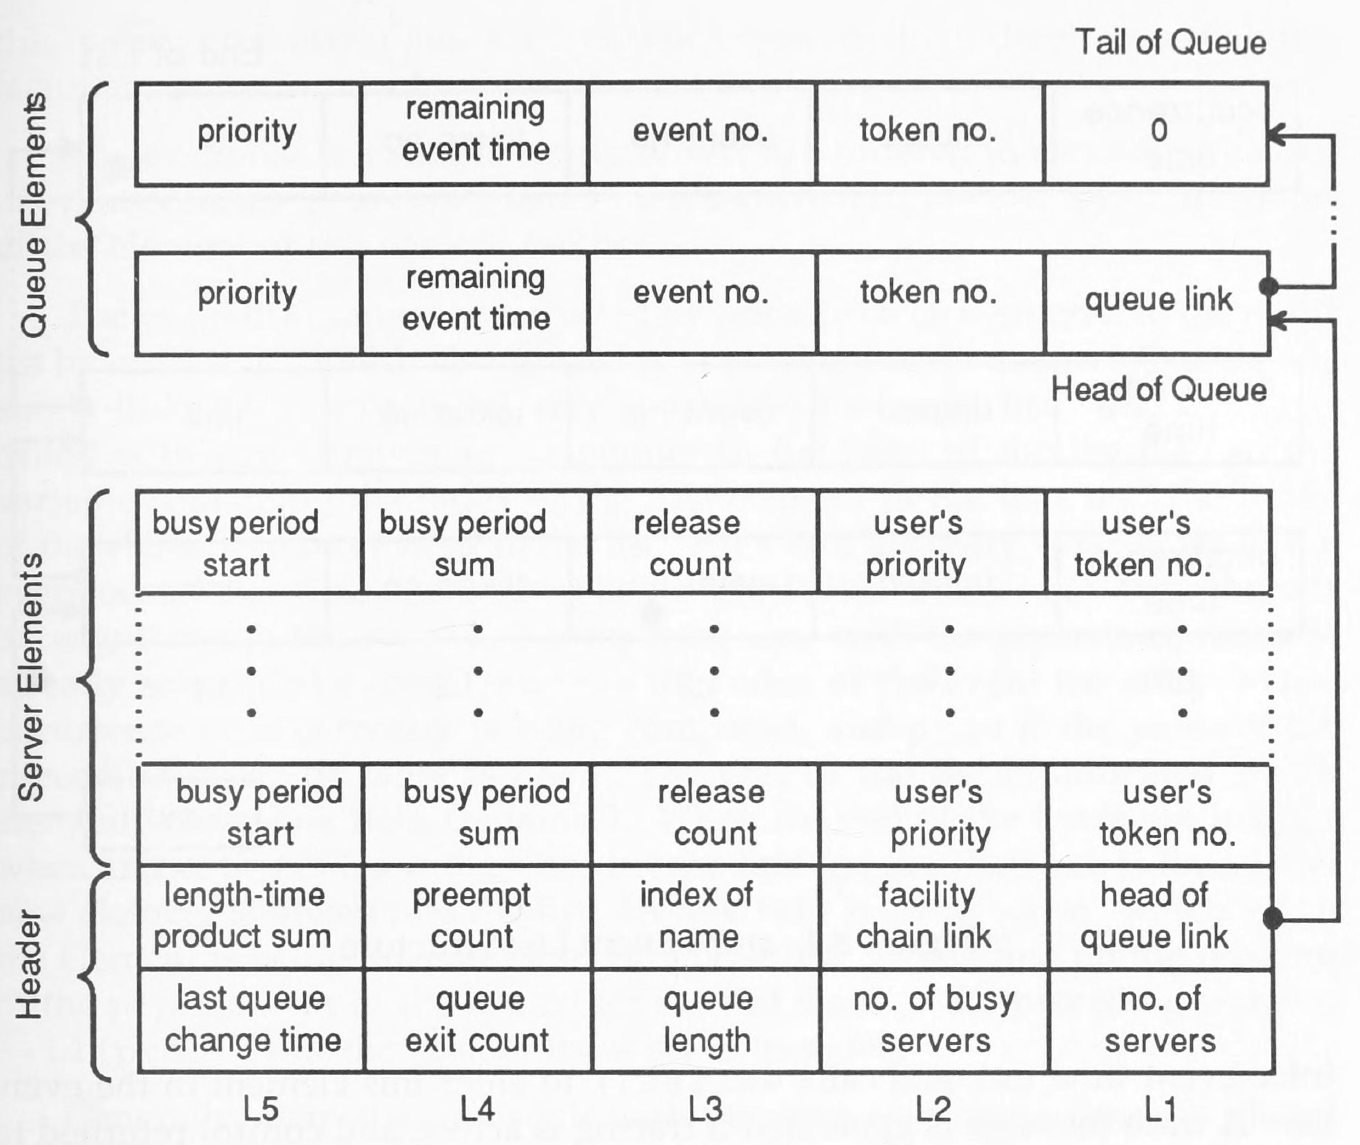
\includegraphics[width=.72\textwidth]{figures/ch8-figure-8-3.png}
\caption{\textbf{smpl} Facility Descriptor and Queue Structure}
\end{figure}

If tracing is active, \texttt{msg()} is called to generate a trace message:
\texttt{fname()} provides a pointer to the facility name. The index of the first
element of the facility descriptor is returned to the caller.

\section{Event Scheduling}

Simulation model initialization includes initializing \textbf{smpl}, defining
facilities, and scheduling the initial events. An event is scheduled via a
call to the \texttt{schedule()} function with parameters \texttt{ev}, \texttt{te}, and \texttt{tkn}. \texttt{ev} is the
event number, \texttt{te} is the inter-event time, and \texttt{tkn} is the token number
associated with the event. After verifying that the inter-event time is not
negative, \texttt{schedule()} calls \texttt{get\_elm()} to get an element from the element
pool, constructs an event list element containing the token number, event
number, and event occurrence time (the sum of the current time \texttt{clock} and the

\OriginalPage{220}{Implementing smpl}
\begin{figure}[H]
\centering
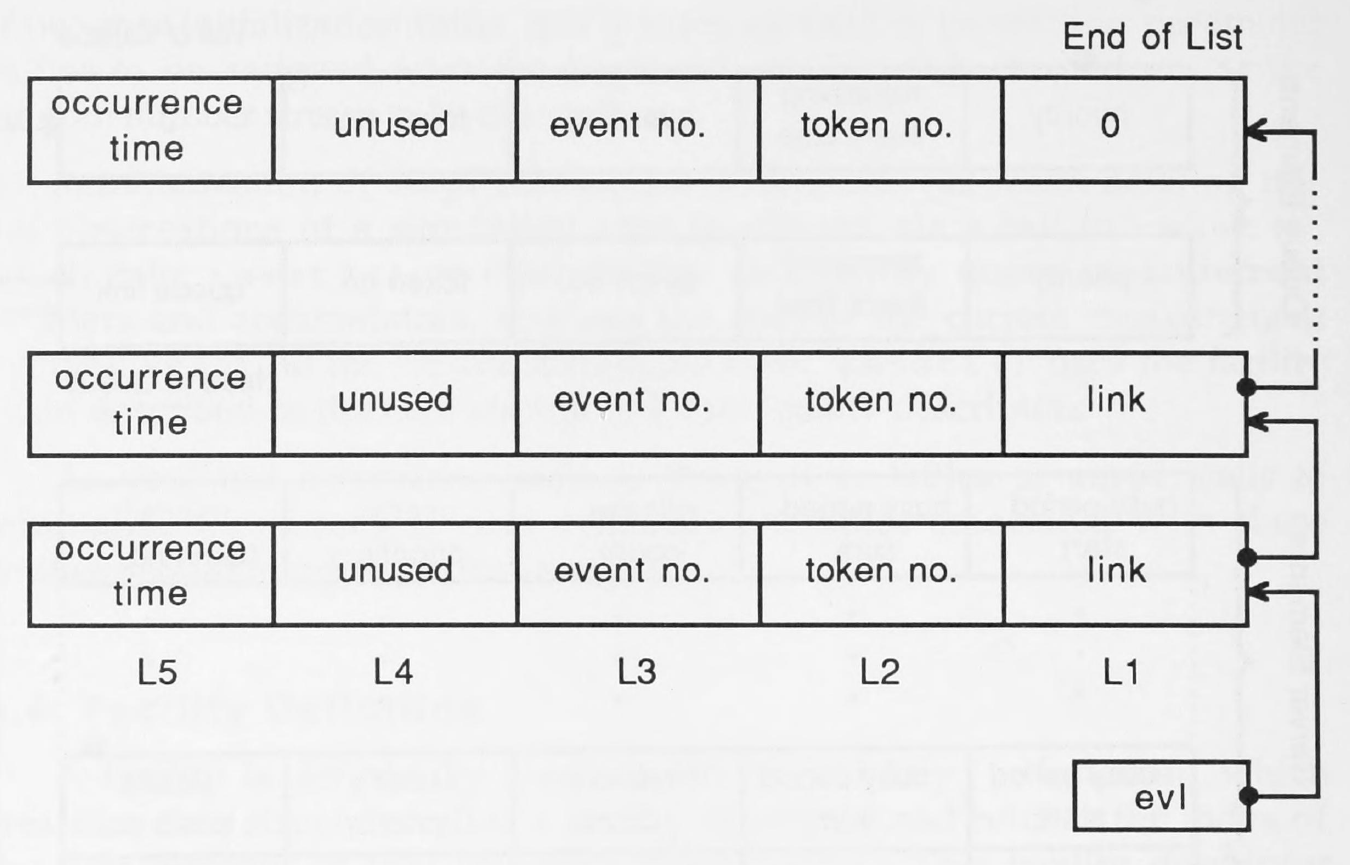
\includegraphics[width=.78\textwidth]{figures/ch8-figure-8-4.png}
\caption{\textbf{smpl} Event List Structure}
\end{figure}

\noindent inter-event time \texttt{te}), and calls \texttt{enlist()} to enter this element in the event
list. A trace message is generated if tracing is active, and control returned to
the user.

\texttt{get\_elm()} allocates a single element from a linked list of available
elements. Before this list can be used, however, it has to be built:
\texttt{get\_elm()} does this the first time it is called. \texttt{smpl()} initializes \texttt{avl} to
$-1$ and \texttt{blk} to 1. As facilities are defined, blocks of elements are allocated
for facility descriptors by \texttt{get\_blk()}, and \texttt{blk} advanced accordingly. \textbf{smpl}
requires that all facilities be defined before the first event is scheduled (or
the first queue entry is made). On the first call to \texttt{get\_elm()}, indicated by
\texttt{avl = -1}, the elements remaining in the pool after facility definition are
linked into a list. \texttt{avl} is set to the index of the element at the head of the
list: the link field of the last element in the list, \texttt{L1[nl]}, is zero, marking
the end of the list. \texttt{blk} is set to zero so that any subsequent call to
\texttt{get\_blk()} will result in an error. After transforming the element pool into
a list (or on calls after the first), \texttt{get\_elm()} unlinks the element at the
head of the list and returns its index to the caller.

When \textbf{mtr} is present (and active), the second \textbf{mtr} initialization call is
made on the first call to \texttt{get\_elm()}. All facilities have been defined at


\OriginalPage{221}{8.5 Event Scheduling}
\noindent this point, and \textbf{mtr} pauses execution again so that displays involving
facilities can be invoked.

The event list is a simple singly-linked list, ordered in ascending values
of event occurrence times; its structure is shown in Figure 8.4. \texttt{evl} is the index
of the element at the head of the list.

The event list element constructed by \texttt{schedule()} is entered in the event
list by \texttt{enlist()}, which also is used to enter elements in queues. Queues are
singly-linked lists structured very much like the event list. \texttt{enlist()} is
called with two parameters: a pointer to the head of the list (i.e., to the
variable containing the index of the first element in the list), and the index
of the element to be entered in the list. For event list entry, \texttt{arg} is set to the
event occurrence time of the event being scheduled. \texttt{enlist()} then threads
its way through the event list, comparing \texttt{arg} with the occurrence times of
already scheduled-events. \texttt{succ} is the index of the event list entry whose
occurrence time currently is being compared, and \texttt{pred} is the index of the
preceding entry (if there is one). The end of the list is indicated by an
element whose link field contains 0. When the end of the list is reached, or
when an existing entry with an occurrence time greater than \texttt{arg} is found, the
new element is linked into the list. Its link field is set to \texttt{succ}, which is 0 if
the element is being linked to the end of the list. Depending on the position
of the new element in the list, either the link field of the preceding element
--- \texttt{L1[pred]} --- or the head of list is set to its index.

Generally, elements for events with the same occurrence time are placed
on the event list in first-in, first-out order. There is one exception: when an
event is rescheduled for a dequeued token which was queued because of a
blocked request or preempt operation, it is placed (directly, by \texttt{release()})
at the head of the event list.

The simulation program calls \texttt{cause()} to obtain the next event to occur
together with the token associated with that event: call parameters are
pointers to the program's event number and token number variables.
\texttt{cause()} verifies that the event list is not empty, returns the token number
and event number from the element at the head of the event list, sets \texttt{event}
to this event number, and sets the current simulation time \texttt{clock} to the event
occurrence time from this element. It then delinks the element from the event
list, calls \texttt{put\_elm()} to return the element to the pool, and generates a trace
message if tracing is active.

\textbf{smpl} uses \texttt{event}, the current event, to keep track of the event routine
currently being executed by the simulation program. If a token's facility
request is blocked or its reservation of a facility is preempted, \textbf{smpl} queues
the token and records the current event in the queue entry. When the token is

\OriginalPage{222}{Implementing smpl}
\noindent dequeued, this event is rescheduled for it. Consequently, the simulation
program should not directly transfer control between event routines: if it
does, \texttt{event} will not be valid.

The \texttt{cause()} function is the primary point of interaction between \textbf{smpl}
and \textbf{mtr}. If \textbf{mtr} is present and active, \texttt{mtr()} is called on every execution of
\texttt{cause()} (unless trace mode 3 has been selected, in which case a monitor
pause occurs after every trace message). \texttt{mtr()} performs any necessary
updates of \textbf{mtr}-initiated displays or analyses (such as \textbf{bma}), checks for and
processes keyboard interrupts (from SMPL function keys), and updates the
simulation time displayed on the screen before returning. We'll take a closer
look at \textbf{mtr} in Chapter 9.

Occasionally, as in the Ethernet model of Chapter 6, events occurring
after a particular event has been scheduled make it necessary to cancel the
occurrence of that event. The \texttt{cancel()} function searches the event list for
event \texttt{ev} and, if an entry for that event is found, unlinks the entry from the
list, deallocates it, and returns the token number from the entry to the caller.
The \texttt{suspend()} function is called by \texttt{preempt()} when a token's use of a
facility is being preempted. \texttt{suspend()} searches the event list for an event
scheduled for that token, unlinks the entry from the list, and returns the
element index of the entry to \texttt{preempt()}.

Event scheduling in \textbf{smpl} is based on a simple singly-linked list about
which Reeves [1984] says ``... it may be thought scandalous if the simple
linear linked list remains in common use ...''. We'll revisit this subject in the
next chapter.

\section{Facility Reservation and Release}

\textbf{Request function processing.} A simulation program makes a non-
preemptive facility reservation request via a \texttt{request()} call: call
parameters are the facility descriptor index \texttt{f}, the requestor's token number
\texttt{tkn}, and the request's priority \texttt{pri}. \texttt{request()} compares the number of busy
servers for the facility, \texttt{L2[f]}, with the total number of servers \texttt{L1[f]}. If
at least one server is free, the server element set is searched for a free server
(a server element whose L1 field is 0); \texttt{i} is set to the index of the free
server's element. The server is reserved by setting \texttt{L1[i]} to the requestor's
token number, and recording the request's priority and the server's current
busy period starting time in the server element. The facility's busy server
count is incremented, and \texttt{r} is set to 0 so that the function return will indicate
to the caller that the facility has been reserved. Note that since a server is
marked busy by setting the L1 field of the server element to the requestor's

\OriginalPage{223}{8.6 Facility Reservation and Release}
\noindent token number, 0 is not a valid token number for facility operations: you may
want to add a check for this in reserve/preempt processing.

If all servers of a facility are busy, \texttt{request()} calls \texttt{enqueue()} to build
a facility queue entry and sets \texttt{r} to 1 so that the function return will indicate
that the request has been blocked. \texttt{enqueue()} call parameters in this case
are the request parameters, the current event \texttt{event}, and the remaining
event time, which is 0 for a blocked request. \texttt{enqueue()} updates the queue
length-time product accumulator \texttt{L5[f+1]},\footnote{This sum, divided by the length of the measurement period, gives the mean queue length: see Section 1.5.}
increments the current queue
length \texttt{L3[f]}, and sets the last queue entry/exit time \texttt{L5[f]} to the current
simulation time. \texttt{get\_elm()} is called to allocate an element from the pool
for the queue entry, and the requestor's token number and priority, the current
event, and the remaining event time are recorded in the entry. \texttt{enlist()} is
called to insert this entry in the facility's queue: call parameters are a
pointer to the head of the queue \texttt{L1[f+1]} (which contains either 0 or the
index of the first element in the queue) and the index of the queue entry.

A facility queue is a singly-linked list ordered in descending priority
values: the highest-priority entry, then, is at the head of the list.
\texttt{enlist()} is used to enter elements in queues as well as in the event list; it
determines where an entry should be inserted by comparing the argument
field L5 of the new entry with those of existing entries. (Note that in
constructing a queue entry, \texttt{enqueue()} converts the request's priority from
\texttt{int} to \texttt{real} in assigning it to L5.) The only difference in \texttt{enlist()}
execution between event list entry and queue entry is in argument comparison:
the event list is ordered in ascending values of L5, queues in descending order.
For a blocked facility request, the entry's L4 field is 0, and \texttt{enlist()} inserts
the entry after existing entries of the same priority.

If tracing is active, \texttt{request()} generates a trace message before
returning to the caller. The trace \texttt{msg()} function uses \texttt{r} to determine if a
reserve or a queue message should be issued.

\textbf{Preempt function processing.} A preemptive facility reservation request is
issued via a call to \texttt{preempt()}: call parameters are the same as those of
\texttt{request()}. When the requested facility is nonbusy, reservation processing
is the same for both preemptive and non-preemptive requests (although the
code is slightly different). The server element set is searched for a free
server, the requestor's token number and priority, together with the busy

\OriginalPage{224}{Implementing smpl}
\noindent period starting time, are recorded in the server element, the busy server count
for the facility is incremented, and 0 is returned to the caller.

If all the servers are busy, \texttt{preempt()} searches the server element set
for the server with the lowest priority user. If the request's priority is not
higher than that of the lowest priority user, the request is queued in just the
same way as a blocked non-preemptive facility request: \texttt{enqueue()} builds
the queue entry, \texttt{enlist()} inserts the entry in the queue, and 1 is returned to
the caller.

If the request's priority is greater than that of the lowest priority user
(whose element index is \texttt{k}), that user is preempted and the facility reserved
for the requestor. This is done as follows.
\begin{enumerate}
\item \texttt{suspend()} is called to search the event list for an entry
with the same token number as the user, unlink the element
from the list, and return its index \texttt{i}. \textbf{smpl} assumes that the
user has one and only event scheduled, and that event represents
completion of the user's current facility reservation.
% Printed page 224 reads "one and only event"; retained as printed.
\item The event number \texttt{ev} of the suspended event is noted and
the remaining event time \texttt{te} --- the difference between the
event occurrence time and the current simulation time --- is
computed. If preemption happens to be taking place at the
same instant in time that the facility was to be released, so
that the remaining event time is 0, \texttt{te} is set to a very small
but non-zero value. \texttt{enlist()} and \texttt{release()} distinguish
between blocked and preempted requests on the basis of zero
or non-zero remaining event times.
\item \texttt{put\_elm()} is called to deallocate the element removed
from the event list, and \texttt{enqueue()} is called to construct a
queue entry for the preempted user. \texttt{enqueue()} calls
\texttt{enlist()} to insert the entry in the queue. In this case, with
\texttt{L4[elm]} (the remaining event time) greater than 0,
\texttt{enlist()} inserts the new queue entry ahead of other entries
of the same priority. Thus, the most recently preempted
request will be returned to execution before other preempted
(or blocked) requests of the same priority. Note that, if
desired, two function calls could be eliminated here by
having \texttt{preempt()} use the element removed from the event
list to build the queue entry and calling \texttt{enlist()} directly
to insert the entry in the queue.
\item The release count \texttt{L3[k]} and busy period sum \texttt{L4[k]} for
the interrupted server are updated, the number of busy

\OriginalPage{225}{8.6 Facility Reservation and Release}
servers \texttt{L2[f]} decremented, and the facility's preempt count
\texttt{L4[f+1]} incremented.
\item The interrupted server is reserved for the requestor.
\end{enumerate}

If tracing is active, trace messages are generated showing the actual
operations performed. Figure 2.3 shows an example of the messages
generated when preemption takes place.

\textbf{Release function processing.} \texttt{release()} is called to release a server of a
facility: call parameters are the facility descriptor index \texttt{f} and the token
number \texttt{tkn} associated with the original reservation. \texttt{release()} searches
the server element set, beginning with element 1, for a server reserved for
\texttt{tkn}: \texttt{j} is the index of this element. An error exit occurs if no element
reserved for \texttt{tkn} is found. Note that the servers of a facility are identical
and indistinguishable; it is possible for multiple servers to be reserved by a
single token (as, for example, when a facility is used to represent a buffer
pool) and selection of a particular server for release essentially is arbitrary.

The server to be released is marked nonbusy by setting L1 of the server
element to 0. The server release count L3 is incremented, the length of the
busy period just completed is computed and added to the server's busy period
accumulator L4, and the number of busy servers for the facility, \texttt{L2[f+1]}, is
decremented. If tracing is active, a trace message is generated and, if the
facility queue is empty, \texttt{release()} then returns to its caller.
% Printed page 225 says L2[f+1], although Figure 8.3 identifies L2[f] as the busy count.

If the facility queue is not empty, \texttt{release()} dequeues the element at
the head of the queue: \texttt{k} is the index of this element. The queue length-time
product accumulator \texttt{L5[f+1]} is updated, the current queue length \texttt{L3[f]}
decremented, the queue exit count \texttt{L4[f]} incremented, and the last queue
entry/exit time \texttt{L5[f]} set to the current simulation time. The dequeued
request may be either a blocked or a preempted facility reservation request:
the remaining event time \texttt{L4[k]} of a blocked request is zero, while that of a
preempted request is greater than zero.

If the dequeued request originally was blocked, \texttt{release()} reschedules
execution of the event routine which originally generated the request
(remember that the current event number was recorded when the queue entry
was made). Queue elements have the token number and event number
recorded in the same fields (L2 and L3) as event list elements; \texttt{release()}
sets the L5 field to the current simulation time and inserts the element at the
head of the event list. This insures that, even though there may be other
requests for the facility scheduled for this same instant in simulation time,
reinitiation of this facility request will be successful since its event routine
will be selected on the next \texttt{cause()} call (provided, of course, that the \mbox{simu-}

\OriginalPage{226}{Implementing smpl}
\noindent lation program itself does not schedule a facility request after the release).
\texttt{m} is set to select a ``reschedule'' trace message.

If the dequeued request is being returned to execution after preemption,
the server just released is reserved for it. The token number and priority are
copied from the element of the dequeued request to the server element (note
that the priority is converted back to \texttt{int} in the process), the server's busy
period start time is set to the current simulation time, and the busy server
count for the facility is incremented. If tracing is active, a ``reserve'' trace
message is generated. The dequeued request's element is used for the event
list entry: \texttt{release()} computes the event occurrence time for the request,
stores it in the L5 field, and calls \texttt{enlist()} to insert the element in the
event list. \texttt{m} is set to select a ``resume'' trace message.

A preempted request is rescheduled for execution at a time equal to its
remaining event time plus the current simulation time. In preemption
processing, if preemption takes place at the same instant in time that the
preempted request was scheduled to release the facility (so that its actual
remaining event time is zero), \texttt{preempt()} sets the remaining event time to a
very small non-zero value. \texttt{release()} doesn't bother to do anything about
this, so the actual facility execution interval in this situation will be very
slightly greater than that scheduled. For most models, this doesn't matter:
the situation rarely occurs, and the small increment has no real effect on
simulation results. There is, however, one class of models for which this
increment is a problem: hardware-level models in which times are
multiples of machine clock cycles, and so are integer-valued (although not
\texttt{int}s). In this case, adding a very small fractional value to an execution
interval can upset model timing. If your applications include models of this
class, you should revise \texttt{release()} to check and correct the remaining event
time.

\section{Facility Query Functions}

The \texttt{status()}, \texttt{inq()}, \texttt{U()}, \texttt{B()}, and \texttt{Lq()} functions return instantaneous
or average facility measures; all are called with the facility
descriptor index \texttt{f} as the single parameter. Operation of these functions
should be clear from looking at the code together with Figure 8.3.

\texttt{status()} returns 1 if all servers of a facility are busy, and 0 otherwise:
some modelers prefer to have it return the number of free servers. The \texttt{U()},
\texttt{B()} and \texttt{Lq()} functions are used in generating the \textbf{smpl} simulation report:
they can be used to generate reports tailored to a particular model, or to
accumulate measures across multiple simulation runs. If you need to develop

\OriginalPage{227}{8.8 Debugging and Reporting Functions}
\noindent model-specific reports, you may want to add functions to return release and
queue exit counts.

\section{Debugging and Reporting Functions}

\textbf{Output and page control.} trace and error messages, and the simulation
report, are directed to the current output destination specified by the file
pointer \texttt{opf} (which is initialized to \texttt{stdout}). The simulation program can
change the output destination (or get the current destination) via a call to
\texttt{sendto()}. The output produced by \textbf{smpl} usually will be sent either to a
printer or to the screen. \textbf{smpl} defines two values, \texttt{pl} and \texttt{sl}, as the number of
output lines which can be written to a printer page or a screen ``page'', and
maintains a variable, \texttt{lft}, which is a count of the number of lines remaining
on the current page. The program can coordinate line counting with \textbf{smpl} by
calling \texttt{trace()} (with a parameter value of 4) to count program-generated
trace lines and \texttt{lns()} to count program-generated output lines.

Page end processing is done by \texttt{endpage()}, which is called by \texttt{lns()}
when there are no more lines left on the current page, and by other functions
on completion of output (e.g., end of report). If the current output destination
is the screen, \texttt{endpage()} pushes the output to the top, displays a message,
and pauses. When the user responds, \texttt{endpage()} clears the screen if \textbf{mtr} is
available and active and otherwise generates an inter-display spacer. If
the current output destination is the printer, \texttt{endpage()} issues a form feed
(if not at top-of-page). Before returning to its caller, \texttt{endpage()} calls
\texttt{newpage()} to reset the line count to top-of-page.

\textbf{Trace functions.} The simulation program calls \texttt{trace()} to turn tracing on
or off, or to count a program-generated trace line. The call parameter \texttt{n}
determines the operation to be performed. Tracing is turned off (\texttt{n = 0}) by
setting the trace control flag \texttt{tr} to 0. It is turned on (\texttt{n = 1--3}) by setting the
trace control flag to \texttt{n}: the last trace message issue time \texttt{tl} is set so that the
first trace message issued will be time-stamped, and \texttt{newpage()} is called to
set the output line count to correspond to top of page or top of screen. (The
simulation program should issue a form feed before initiating a trace when
output is to the printer.)

Trace messages are generated via calls to \texttt{msg()} made by various
simulation functions when tracing is active. Call parameters are a message
number \texttt{n}, an optional token number \texttt{i}, a character string pointer \texttt{s}, and
qualifying parameters \texttt{q1} and \texttt{q2} (which provide additional information,
such as event numbers and current queue lengths). A trace message comprises
four segments:

\OriginalPage{228}{Implementing smpl}
\begin{figure}[H]
\centering\footnotesize\ttfamily
\resizebox{\textwidth}{!}{%
\begin{tabular}{lllllll}
\multicolumn{5}{c}{parameters} & \multicolumn{2}{c}{message phrase}\\
n & i & s & q1 & q2 & string - m[n] & qualifier\\\hline
1 & tkn & 0 & ev & 0 & SCHEDULE & EVENT q1\\
2 & tkn & 0 & ev & 0 & CAUSE & EVENT q1\\
3 & tkn & 0 & ev & 0 & CANCEL & EVENT q1\\
4 & -1 & 0 & ev & 0 & RESCHEDULE & EVENT q1\\
5 & -1 & 0 & ev & 0 & RESUME & EVENT q1\\
6 & -1 & 0 & ev & 0 & SUSPEND & EVENT q1\\
7 & tkn & *fn & 0 & 0 & REQUEST & : RESERVED\\
7 & tkn & *fn & 1 & L3[f] & REQUEST & : QUEUED (inq=q2)\\
8 & tkn & *fn & 0 & 0 & PREEMPT & : RESERVED\\
8 & tkn & *fn & 1 & L3[f] & PREEMPT & : QUEUED (inq=q2)\\
8 & tkn & *fn & 2 & 0 & PREEMPT & : INTERRUPT\\
9 & tkn & *fn & 0 & 0 & RELEASE & \\
10 & -1 & 0 & tn & L3[f] & QUEUE & token q1 (inq=q2)\\
11 & -1 & 0 & tn & L3[f] & DEQUEUE & token q1 (inq=q2)\\
12 & -1 & *fn & tn & 0 & RESERVE & for token q1\\
13 & -1 & *fn & f & 0 & FACILITY & : f=q1
\end{tabular}}
\caption{Trace Message Parameters and Phrases}
\end{figure}

\begin{center}
$\langle$time stamp$\rangle$ $\langle$token number$\rangle$ $\langle$basic message$\rangle$ $\langle$qualifier$\rangle$
\end{center}

The time stamp segment is generated only when the current simulation time
is greater than the time (\texttt{tl}) at which the last message was generated. The
token number segment is generated only when \texttt{i} is non-negative. The basic
message is formed by concatenating the message phrase string \texttt{m[n]} and the
parameter string \texttt{s} (which is null for some messages). For most messages, a
qualifier is appended: its form depends on the message number and, for
facility request and preempt operations, on the value of \texttt{q2}.

Figure 8.5 shows the various \texttt{msg()} parameter combinations and the
corresponding message phrase strings and qualifiers. In this figure, \texttt{tkn}
represents a token number, \texttt{ev} represents an event number, and \texttt{*fn} represents
a facility name pointer. \texttt{f} is a facility descriptor index, and \texttt{L3[f]} is the
current queue length field from the facility descriptor. The trace message
sequence of Figure 2.3 shows most of the message formats.

\texttt{end\_line()} is called by \texttt{msg()} after a \textbf{smpl} trace message has been
printed and by \texttt{trace()} when the latter is called to count a program-
generated trace line (i.e., with \texttt{n = 4}). It decrements the line counter \texttt{lft}
and, if the count is reduced to zero, performs page end processing as \mbox{deter-}


\OriginalPage{229}{8.9 Random Variate Generation}
\noindent mined by the trace mode. In trace mode 1, \texttt{endpage()} is called to generate a
form feed if output is not to the screen: otherwise, the line count simply is
reset (in this mode, output to the screen is generated without pause). In trace
mode 2, \textbf{smpl} pauses execution on each full screen: if \textbf{mtr} is available and
active, \texttt{pause()} is called to initiate a monitor pause. In the absence of \textbf{mtr},
\texttt{endpage()} is called to pause execution for screen output or generate a form
feed for printer output. In trace mode 3, execution is paused after each trace
message is printed.

\textbf{Error processing.} When \textbf{smpl} detects an error, such as an empty event list,
it calls \texttt{error()} to issue a diagnostic message, print the simulation report (if
output is to the printer), and halt execution. This function also can be called
from the simulation program if desired. \texttt{error()} is called with two parameters:
an error number \texttt{n} and a character string pointer \texttt{s}. For errors detected
by the functions in \textit{smpl.c}, \texttt{error()} is called with \texttt{n = 1--8} and \texttt{s} null. For
errors detected by other modules (such as \textit{rand.c} or the simulation program),
it is called with \texttt{n = 0} and \texttt{s} pointing to a diagnostic message.

If the current output destination is the printer, \texttt{error()} sends the error
message both to the screen and the printer, and prints the simulation report.
If \textbf{mtr} is available and active, a monitor pause is initiated. This provides an
opportunity to examine various displays, such as the simulation dump or
report, before execution is terminated via a call to \texttt{exit()}.

\textbf{Report generation.} The simulation report is generated by a call to
\texttt{report()} from the simulation program or from \texttt{error()}. In this version of
\textbf{smpl}, \texttt{report()} simply calls \texttt{reportf()} to produce the facility report; in
an extended version, \texttt{report()} might include calls to generate table or
storage reports. Note that you can call \texttt{reportf()}, rather than \texttt{report()},
to avoid the form feed or screen pushup generated by \texttt{endpage()}.

\texttt{reportf()} traces the facility chain constructed by \texttt{facility()}, and
calls \texttt{rept\_page()} until the end of the chain is reached. \texttt{rept\_page()}
prints the report heading, followed by a report line for each facility, until
the page is full or the chain end reached. Generation of the facility report
lines is straightforward: review the code together with Figure 8.3. Figure
2.4 shows an example of the simulation report format.

\section{Random Variate Generation}

\textbf{smpl} random variate generation functions are contained in the \textit{rand.c}
file: a listing for this file follows that of \textit{smpl.c} in the Appendix. \textit{rand.c}
function names are listed in Figure 8.6: all of these functions can be called
from the simulation program.


\OriginalPage{230}{Implementing smpl}
\begin{figure}[H]
\centering\small
\begin{tabular}{@{}lp{.65\textwidth}@{}}
\texttt{ranf()} & generate uniform random variate\\
\texttt{stream()} & set/get random number stream\\
\texttt{seed()} & set/get seed for stream n\\
\texttt{random()} & generate random integer\\
\texttt{expntl()} & generate exponentially-distributed random variate\\
\texttt{erlang()} & generate Erlang-distributed random variate\\
\texttt{hyperx()} & generate hyperexponentially-distributed random variate\\
\texttt{normal()} & generate normally-distributed random variate
\end{tabular}
\caption{\textit{rand.c} Functions}
\end{figure}

\textbf{Uniform random variate generation.} \textbf{smpl} uses the venerable multiplicative
congruential random number generator
\begin{equation}
I_{n+1}=\alpha I_n\ \bmod\ M
\end{equation}
with $\alpha=7^5=16807$ and $M=2^{31}-1=2147483647$ (a prime). It has a period
(number of values generated before the sequence repeats) of $M-1$. This
generator originally was described by Lewis et al [1969], and has been
extensively tested (testing results can be summarized as ``good: not great'').
It is discussed in our simulation texts and by Kobayashi [1978]. A frequently-
referenced implementation is called LLRANDOM [Learmonth and Lewis
1973].

\textbf{smpl}'s random number generator function, \texttt{ranf()}, uses the recursion of
(8.1) to generate integer variates uniformly distributed in the range $1$, $M-1$,
then converts these to floating-point variates uniformly distributed in $0+\epsilon$,
$1-\epsilon$ (where $\epsilon$ is a very small value). Both of the arithmetic operations
required to compute $I_{n+1}$ present problems: the divide operation frequently is
very slow, and the multiply operation usually requires double precision.

The use of division to perform the modulo operation in (8.1) can be
avoided using the simulated division method described by Payne et al [1969].
(This method also is described in several of our simulation texts, by
Kobayashi [1979], and by Schrage [1979].) The method works as follows.
Define
\begin{equation}
Z=16807I_n\ \bmod\ 2^{31}
\end{equation}

\OriginalPage{231}{8.9 Random Variate Generation}
\begin{figure}[H]
\centering
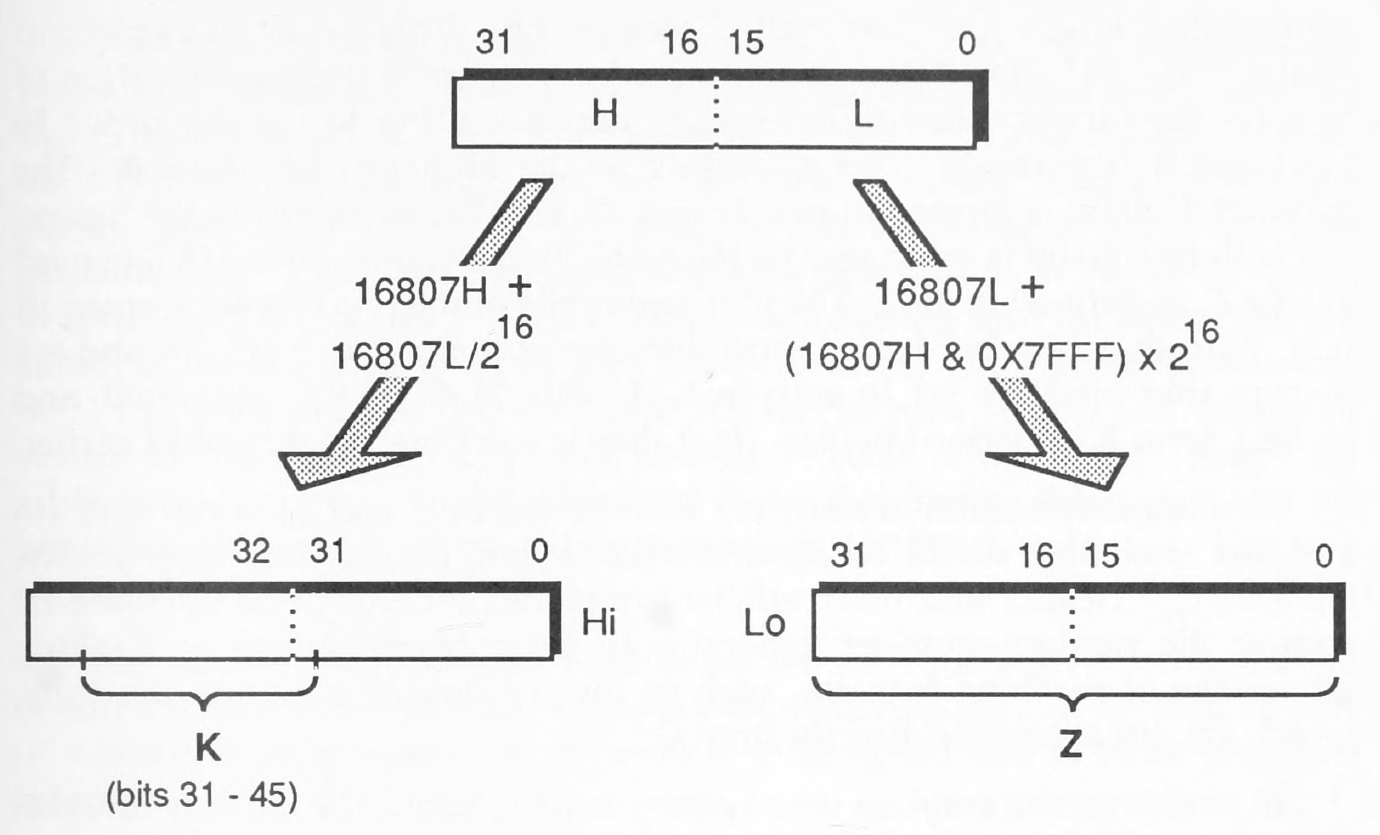
\includegraphics[width=.9\textwidth]{figures/ch8-figure-8-7.png}
\caption{Simulated Double Precision Multiply Operands and Operations}
\end{figure}

\noindent and
\begin{equation}
K=\lfloor 16807I_n/2^{31}\rfloor
\end{equation}
where $\lfloor x\rfloor$ denotes the floor function of $x$ --- the largest integer equal to or less
than $x$. The product $16807I_n$ comprises a maximum of 46 bits: $Z$ represents the
low-order 31 bits and $K$ represents the higher-order bits, treated as a number.
It can be shown (see the references cited above) that
\begin{equation}
\begin{aligned}
I_{n+1}&=Z+K, &&\text{if }Z+K<M\\
I_{n+1}&=Z+K-M, &&\text{if }Z+K>M
\end{aligned}
\end{equation}
% Equation 8.4 uses >, not >=, in the second condition in the printed source.

In implementing (7.4) with 32-bit arithmetic, $M$ should be pre-subtracted
from $Z$ to avoid possible overflow: that is, compute $Z-M+K$ (in that order:
you may have to outwit your compiler) and, if the result is less than zero,
add $M$ back in to form $I_{n+1}$.
% The printed source refers to (7.4), although the immediately preceding equation is (8.4).

For many systems, \texttt{long}s are 32 bits and \texttt{int}s are either 16 or 32 bits in
length: consequently, formation of the 46-bit product $16807I_n$ requires a
double precision integer multiply. The versions of \texttt{ranf()} in the Appendix
are designed for systems with 32-bit \texttt{long} and 16-bit \texttt{short} integers, and use

\OriginalPage{232}{Implementing smpl}
\noindent a simulated double precision multiply to generate this product. The method
is illustrated in Figure 8.7. The \texttt{long} seed is viewed as the concatenation of
two 16-bit \texttt{short}s called \texttt{L} (the integer corresponding to the low-order 16
bits) and \texttt{H} (the integer corresponding to the higher-order 16-bits). The
product $16807I_n$ is formed in two \texttt{long}s, \texttt{Lo} and \texttt{Hi}, as shown in the figure.
\texttt{Lo}, with its sign bit is set to zero by the mask \texttt{0X7FFF}, is equal to $16807I_n$ mod
$2^{31}$, or $Z$, as defined in (8.2). The high-order bits of the product are formed in
\texttt{Hi}: note that bits 16-31 of the product are contained in both \texttt{Lo} and \texttt{Hi}
(except that bit 31 is set to zero in \texttt{Lo}). Bits 31-45 of \texttt{Hi}, extracted and
shifted, form $K$ as defined in (8.2). $I_{n+1}$ then is computed as described earlier.
% Printed page 232 says "with its sign bit is set" and refers to (8.2) for K; retained.

This implementation of \texttt{ranf()}, while coded in C and semi-portable (to
systems with the stated \texttt{long} and \texttt{short} lengths), is not very pretty.
Generally, a cleaner and more efficient implementation can be obtained by
coding the random number generator in assembly language and taking
advantage of machine features, such as integer double precision multiply,
which are not accessible directly from C.

In implementing \textbf{smpl} on your system, \texttt{ranf()} should be the only function
that requires changes. \textit{rand.c} contains two versions of \texttt{ranf()}: one for CPUs
of or similar to the Intel 808x family, and one for CPUs of or similar to the
Motorola 680x0 family. Both versions assume 32-bit \texttt{long} and 16-bit \texttt{short}
integers: however, the relative positions of \texttt{Hi} and \texttt{Lo} are different in the
two families and require different pointer access.

Your math library may provide a random number generator function
(usually called \texttt{rand()}) which you may elect to use in place of \texttt{ranf()}.
This will require replacing \texttt{ranf()} calls with \texttt{rand()} calls in the other random
variate functions of \textit{rand.c}, and revising stream and seed handling.
Before deciding to use the library's random number generator, find out what
algorithm is used. It is not uncommon for library generators to use shift-and-
add generators because of their speed; however, generators of this type show
departures from randomness (see Chapter 8 in Fishman [1978]). If you decide
to implement \texttt{ranf()}, the two sequences listed below will help check your
implementation.
\begin{center}
\begin{tabular}{lrr}
starting seed $I_0$ & 1 & 1973272912\\
$I_1$ & 16807 & 1207871363\\
$I_2$ & 282475249 & 531082850\\
$I_3$ & 1622650073 & 967423018
\end{tabular}
\end{center}
If your random number generator is functionally identical to \texttt{ranf()}, and
identical seeds are used, your simulations of the M/M/1 and central server
queueing models should produce results identical to those presented in
Chapters 1 and 2.


\OriginalPage{233}{8.9 Random Variate Generation}
\textbf{Seeds and streams.} The \texttt{In[]} array declared at the start of \textit{rand.c}
provides seeds for 15 different random number streams; \texttt{strm} is the index of
the currently-selected stream. \texttt{strm} is initialized to 1, and can be changed
via a call to the \texttt{stream()} function (which also can be used to obtain the
current stream index). \texttt{ranf()} uses the current value of \texttt{In[strm]} to
generate a new random variate and stores the new variate in \texttt{In[strm]} prior
to converting it to a \texttt{real} in $[0,1]$. Thus, each starting seed initiates a unique
subset of the sequence generated by the recursion of (8.1). Starting seeds for
the 15 streams are taken from Table A.2 in Fishman [1978], and represent
values of the generator sequence spaced 100,000 values apart. Seeds for
additional streams can be obtained from Fishman's Table A.2 (which
provides 400 seeds) or by extracting every 100,000th value of \texttt{In[15]}
produced by \texttt{ranf()}.

The \texttt{seed()} function is called to set the seed for a given stream or to
obtain a stream's current seed. Its uses include saving the current seed as part
of a model's state when a simulation is interrupted and is to be restarted
later.

\textbf{Uniform variate and random integer generation.} \texttt{ranf()} returns a \texttt{real}
value uniformly distributed in $[0,1]$; \texttt{uniform()} simply maps this value into
the range $[a,b]$. \texttt{random()} works in much the same way, but deals with
integer, rather than real, values.

\textbf{Exponential, Erlang, and hyperexponential variate generation.} The
\texttt{expntl()} function returns a variate from a negative exponential distribution
with mean \texttt{x}: its implementation was discussed in Section 1.2.
\texttt{erlang()} returns a variate from a Erlang distribution with mean \texttt{x},
standard deviation (approximately) \texttt{s}, and number of stages $k=\lfloor x/s\rfloor^2$. A $k$-
stage Erlang-distributed random variable with mean $X$ can be viewed as the
sum of $k$ exponentially-distributed random variables, each with mean $X/k$.
This suggests the following approach to generating Erlang-distributed
variates. Define $v$ as a random variate from a $k$-stage Erlang distribution
with mean $X$ and define $y$ as a random variate from an exponential
distribution with mean $X/k$. Then,
\begin{equation}
v=\sum_{i=1}^{k} y_i
\end{equation}
\begin{equation}
v=\sum_{i=1}^{k} -(X/k)\ln r_i
\end{equation}

\OriginalPage{234}{Implementing smpl}
\noindent where $r_i$ is the uniform random variate from \texttt{ranf()} used to produce $y_i$.
Since $\ln a+\ln b=\ln ab$,
\begin{equation}
v=-(X/k)\ln\left(\prod_{i=1}^{k}r_i\right)
\end{equation}
\texttt{erlang()} computes \texttt{k} from the specified mean and standard deviation and
then computes a variate value using (8.7). When \texttt{x/s} is not integer-valued,
the standard deviation of values produced by \texttt{erlang()} will be less than \texttt{s}.

The \texttt{hyperx()} function returns a variate from a two-stage hyper-
exponential distribution with mean \texttt{x} and standard deviation \texttt{s}. The distribution
sampled by this function is a special case of a two-stage hyper-
exponential distribution, described by Morse [1963]: it requires only two
parameters (mean and standard deviation) for characterization. The
cumulative distribution function for this distribution is
\begin{equation}
\Pr[s\le x]=1-pe^{-2px/X}-(1-p)e^{-2(1-p)x/X}
\end{equation}
where $X$ is the distribution's mean. The squared coefficient of variation $c^2$ is
\begin{equation}
c^2=[1-2p(1-p)]/[2p(1-p)]
\end{equation}
and the standard deviation is $cX$. This distribution can be viewed as being
produced by a mechanism which has two parallel stages. Stage 1, selected
with probability $p$, generates an exponential variate with mean $X/2p$; stage
2, selected with probability $1-p$, generates an exponential variate with
mean $X/[2(1-p)]$. We can use this approach to generate variates from this
distribution. By appropriately specifying $p$, any desired standard deviation
(equal to or greater than $X$) can be obtained. Alternatively, we can specify
the standard deviation and compute the value of $p$ required to produce it.
The coefficient of variation $c$ is equal to the standard deviation divided by
the mean; solving (8.9) for $p$ gives
\begin{equation}
p=[1-[(c^2-1)/(c^2+1)]^{1/2}]/2
\end{equation}
\texttt{hyperx()} computes the coefficient of variation and uses it to compute $p$, uses
$p$ to randomly select one of two exponential distributions, and returns a
variate from the selected distribution.

\texttt{hyperx()} has several drawbacks: it is slow, and it represents only one
member of the family of two-stage hyperexponential distributions. In any
particular application, it is much faster to precompute $c$, $p$ and the stage

\OriginalPage{235}{8.10 The smpl.h File}
\noindent means, so that variate generation simply requires random selection of one
stage mean or the other as the mean of an exponentially distributed variate.
Some form of gamma distribution generation variate function (described in
most of our simulation texts) will provide more representational flexibility.
However, \texttt{hyperx()} does have one virtue: it requires specification of only
the mean and standard deviation. With \texttt{erlang()}, \texttt{expntl()}, and
\texttt{hyperx()}, variates can be generated from distributions with coefficients of
variation less than one, equal to one, and greater than one, using only the
mean and standard deviation to characterize the distribution.

\textbf{Normal variate generation.} \texttt{normal()} returns a variate from a normal
distribution with mean \texttt{x} and standard deviation \texttt{s}. It generates a unit
normal variate using the polar method of Marsaglia and Bray [1964] (see
Section 7.3.6 in Law and Kelton [1982]). This method generates a pair of unit
variates, and so is invoked only on alternating calls. A unit variate is transformed
into a variate from the specified distribution by multiplying it by
the distribution's standard deviation and adding the mean.

\section{The \textit{smpl.h} File}

The \textit{smpl.h} file is intended to be included in all \textbf{smpl} simulation
programs. It provides \texttt{\#include}s for \textit{stdio.h} and \textit{math.h}, \texttt{typedef} and
\texttt{\#define} definitions for \texttt{real} and \texttt{then}, and \texttt{extern} declarations for those
\textbf{smpl} functions which return other than an integer value. As you add functions
to the simulation subsystem, add the appropriate declarations to
\textit{smpl.c}.
% The printed page names smpl.c here, although this paragraph discusses smpl.h.

\section{Summary}

We've examined the workings of the \textbf{smpl} simulation subsystem in
considerable --- perhaps tedious --- detail. An intimate understanding of how
\textbf{smpl} works helps avoid modeling errors and puts you in control of your
simulation environment: if you don't like the way something works, you can
change it!

In implementing your version of \textbf{smpl}, it is best to start with a straight
copy of the source code as listed in the Appendix, changing only \texttt{ranf()} if
necessary. If your version of \texttt{ranf()} is functionally the same as the
Appendix version and uses the same initial seed for stream 1, you should
obtain results for the M/M/1 queue and central server queueing network
simulations identical to those presented in earlier chapters. If you do not,
analyzing trace sequences for these models should provide some insight into
the problem; first, however, determine that it is a functional problem and

\OriginalPage{236}{Implementing smpl}
\noindent not a report generation error. If you use a different random number generator,
results will agree only in a statistical sense, so don't be concerned if there is a
difference between your results and the book's results for a single run. To
verify your implementation, use simple M/M/1 queue and preemptive priority
queue models with known analytic solutions, set parameters to obtain
moderate utilizations, and compare simulation and analytic results using the
methods described in Chapter 4. Once you've checked your implementation,
revisions to match your programming style and environment can be made
more confidently. However, before making substantial revisions, take a look
at the extensions discussed in the next chapter to see if and how they would
fit in your revised subsystem.
